\documentclass[letter,12pt]{report}
\usepackage[top=1in, bottom=1in, left=1in, right=1in]{geometry}

%	Formato
\usepackage[table,xcdraw]{xcolor}
\usepackage{tikz}
\usepackage{fontspec}
\usepackage{titlesec}
\usepackage{graphicx}
\usepackage{fancyhdr}
\usepackage{enumitem}
\usepackage{caption}
\usepackage{newfloat}
\usepackage{hyperref}
\usepackage{array}
\usepackage{tabu}
\usepackage{tabulary}
\usepackage{tabularx}
\usepackage{multirow}
\usepackage{blindtext}
\usepackage[utf8]{inputenc}
\usepackage[document]{ragged2e}
\usepackage{setspace}
\usepackage{makecell}
\usepackage{amsmath}
\usepackage{lscape}
\usepackage{listings}
\usepackage{chngcntr} % Paquete para cambiar la numeración de página
% para el example box
\usepackage[most]{tcolorbox}
\usepackage{pdfpages} %para incluir pdf

\usetikzlibrary{calc}
\usepackage[normalem]{ulem}
\useunder{\uline}{\ul}{}

%	Segun APA, deberia haber ese inicio en el parrafo
% \setlength{\parindent}{0pt}

%	Adapta la linea sin el guion
% \tolerance=1
% \emergencystretch=\maxdimen
% \hyphenpenalty=10000
% \hbadness=10000

%	Nuevos Comandos
\newcommand{\tightlist}{}
\newcommand{\monografia}{$monografia$}
\newcommand{\autor}{$autor$}
\newcommand{\subtitle}{$subtitle$}
\newcommand{\chapuppercase}[1]{\MakeUppercase{#1}}

%	Definiciones de tablas
\newcolumntype{Y}{>{\centering\arraybackslash}X}

\usepackage{titletoc} % Paquete para modificar el ToC
\titlecontents*{chapter}% <section-type>
  [0pt]% <left>
  {}% <above-code>
  {\bfseries\chapuppercase{\chaptername\ \thecontentslabel}\quad}% <numbered-entry-format>
  {}% <numberless-entry-format>
  {\bfseries\hfill\contentspage}% <filler-page-format>

% Definición del comando \mybox para crear cuadros de texto personalizados
\newcommand{\mybox}[4]{%
    \begin{tcolorbox}[%
        enhanced,        % Permite opciones avanzadas de tcolorbox
        colback=gray!10,     % Color de fondo del cuadro
        colframe=black,    % Color del borde del cuadro
        arc=1.5mm,        % Redondeo de esquinas
        title={\bfseries\textcolor{black}{#1}},     % Título del cuadro
        fonttitle=\bfseries, % Estilo del título del cuadro
        top=0.5in,  % espaciado entre el titulo y el cuerpo
        attach boxed title to top left={xshift=1.5em,yshift=-\tcboxedtitleheight/2+2pt}, % Posición del título con ajuste de espaciado
        boxed title style={colback=gray!40, colframe=black, size=small} % Estilo del título del cuadro
        ]
    #4 % Contenido del cuadro
    \end{tcolorbox}%
}

%	Titulos
\setcounter{tocdepth}{5}
\setcounter{secnumdepth}{6}

%	Fondo
\fancypagestyle{plain}{
}
\definecolor{titulo}{HTML}{1f4e79}
\definecolor{navy}{HTML}{0a3257}
\definecolor{azulmargen}{HTML}{1f4f78}
\definecolor{codeblue}{HTML}{3500FA}
\definecolor{codegreen}{HTML}{008116}
\definecolor{codelightblue}{HTML}{1a7e97}
\definecolor{codered}{HTML}{a81a1c}
\definecolor{codebrown}{HTML}{7a5f2c}
\definecolor{codelightgreen}{HTML}{00865a}
\definecolor{codeback}{rgb}{0.95,0.95,0.92}

\newfontfamily{\codefont}[]{JetBrains Mono}
\title{$title$}

\lstdefinestyle{csharpStyle}{
    language=[Sharp]C,   
    backgroundcolor=\color{codeback}, 
    extendedchars=true,
    basicstyle=\codefont\footnotesize,
    showstringspaces=false,
    showspaces=false,
    numbers=left,
    numberstyle=\footnotesize,
    numbersep=9pt,
    tabsize=2,
    breaklines=true,
    showtabs=false,
    captionpos=b,
    keywordstyle=\color{codeblue}\bfseries,
    ndkeywordstyle=\color{codelightblue}\bfseries,
    identifierstyle=\color{codegreen},
    numberstyle=\color{codelightgreen},
    commentstyle=\color{codebrown}\ttfamily,
    stringstyle=\color{codered}\ttfamily
}

\lstset{style=csharpStyle}

%	Colores

\definecolor{sp1}{HTML}{D9E1F2}
\definecolor{sp2}{HTML}{d0c3b4}
\definecolor{sp3}{HTML}{f1f2f2}

%	Bibliografia
\usepackage{csquotes}
\usepackage[spanish,es-noshorthands]{babel} 
\usepackage[style=apa, sortcites=true, backend=biber]{biblatex}
\addbibresource{bibliografia.bib}

\DeclareFloatingEnvironment[fileext=loc,listname={Índice de Códigos},name=Código,]{code}
\captionsetup[code]{name={Código}}

% Espacio entre lineas
\linespread{1.5}

\begin{document}

%Titulos
\titleformat{\chapter}[block]{\normalfont\large\bfseries}{Capítulo \Roman{chapter} }{0em}{\newline}
\titlespacing*{\chapter}{0pt}{-1em}{1em}
\titleformat*{\section}{\bfseries}
\titleformat*{\subsection}{\bfseries}
\titleformat*{\subsubsection}{\bfseries}
\titleformat{\paragraph}[block]{\normalfont\normalsize\bfseries}{\theparagraph}{10pt}{}
\titleformat{\subparagraph}[block]{\normalfont\normalsize\bfseries}{\thesubparagraph}{10pt}{}

%Encabezado de Pagina
\makeatletter
\pagestyle{fancy} %Esta línea establece que se va a utilizar el estilo de encabezado y pie de página definido por fancyhdr.
\fancyhf{} % Esta línea limpia cualquier configuración previa de encabezados y pies de página.
\renewcommand{\headrulewidth}{2pt}% Esta línea define el grosor de la línea que separa el encabezado del cuerpo del texto.
\fancyhead[C]{\leftmark} %Centrar el titulo del encabezado
\fancyfoot[R]{\thepage} %Centrar numeros de pagina en la parte inferior de la hoja

% Definición de encabezado y pie de página para el estilo fancy
\fancypagestyle{plain}{
    \fancyhf{} % Limpiar los encabezados y pies de página
    \renewcommand{\headrulewidth}{0pt} % Elimina la línea horizontal en el encabezado
    \fancyfoot[R]{\thepage} % Números de página en la parte inferior derecha
}

% Después de la carátula, cambiar la numeración de página a números romanos
\let\oldpagenumbering\pagenumbering
\renewcommand{\pagenumbering}[1]{%
  \oldpagenumbering{#1}%
  \ifthenelse{\equal{#1}{roman}}{\setcounter{page}{1}}{}%
}

\begin{titlepage}
\begin{singlespace}
	
	\tikz[remember picture,overlay] \node[inner sep=0pt] at (8.3,-7){
\includegraphics[scale=0.25]{Escudo_FICCT.png}};

	\begin{center}
		\vspace{-1.8em}
		\textbf{\large {UNIVERSIDAD AUTÓNOMA GABRIEL RENÉ MORENO}}\\[1em]
		\textbf{{FACULTAD DE INGENIERÍA EN CIENCIAS DE LA COMPUTACIÓN Y TELECOMUNICACIONES}}\\[1em]
		\textbf{UAGRM SCHOOL OF ENGINEERING}\\[1em]
		
		
		\makeatletter
		\vspace*{21em}
		\textbf{\large \@title}\\[2em]
		\textbf{\Large \subtitle}\\[2em]
				
		
		\textbf{\large \monografia}\\[2em]
		\textbf{\large Autor:} {\large \autor}\\[1em]
	
				
		\vfill
		\textbf{Santa Cruz de la Sierra - Bolivia}\\[0.5em]
		\textbf{Mayo, 2024}
		
	\end{center}
\end{singlespace}
\end{titlepage}

\pagenumbering{roman} % Numeración romana para las páginas preliminares
\begingroup
\pagestyle{plain}
\clearpage
\pagenumbering{roman} 
    \setcounter{page}{1}
\thispagestyle{plain}
\section*{\centering DEDICATORIA}
\justify % Texto justificado

Dedico este trabajo con profunda gratitud a las personas que han iluminado mi camino y me han impulsado a alcanzar mis metas. \newline

A mi Padre, Julio César Montaño Toledo, por su apoyo incondicional y su fe inquebrantable en mis capacidades. Su guía y aliento han sido pilares fundamentales en mi formación personal y profesional. \newline

A mi Madre, Marcela Pérez Flores (+), A su memoria eterna dedico este logro. Su amor infinito y su ejemplo de perseverancia me han inspirado a seguir adelante en los momentos más difíciles. Su presencia vive en mi corazón y me motiva a ser una mejor persona cada día. \newline

A mi Tía, Roxana Peña, Agradezco inmensamente su cariño y apoyo incondicional. Ha sido como una segunda madre para mí, brindándome siempre un refugio seguro y un faro de esperanza. \newline

A mis Hermanas, Dulce María y Sofía, su amor, apoyo y compañía han sido esenciales en mi vida. Espero serles un ejemplo de perseverancia y dedicación. \newline

A mi fiel compañero, mi perrito, Copito de Nieve, quien me llena de incondicional amor y alegría. Su presencia en mi vida me llena de felicidad y me recuerda la importancia de disfrutar cada momento. \newline

Con Amor y Gratitud, \newline
Yuliana
\clearpage
\clearpage
\pagenumbering{roman} 
    \setcounter{page}{2}
\thispagestyle{plain}
\section*{\centering RESUMEN}
\justify % Texto justificado
El presente trabajo explora estrategias para fomentar una cultura DevOps y mejorar la implementación de prácticas de Integración Continua (CI) y Entrega Continua (CD) en equipos de desarrollo de software. DevOps se define como un enfoque cultural y metodológico que busca integrar y optimizar el flujo de trabajo entre los equipos de desarrollo y operaciones, promoviendo la colaboración, comunicación y automatización. \newline

En el capítulo de antecedentes y contextualización, se destaca la evolución histórica de DevOps y su relevancia actual en la industria del desarrollo de software. Se analiza cómo DevOps aborda los desafíos de colaboración entre equipos y mejora la eficiencia en el ciclo de desarrollo, haciendo un paralelo con la revolución manufacturera de la década de 1980 y la adopción de principios Lean.\newline

En el marco teórico, se explican los fundamentos y principios de DevOps, incluyendo las tres vías fundamentales: pensamiento de flujo/sistemas, amplificación de los bucles de retroalimentación y una cultura de experimentación y aprendizaje continuo. Además, se describen las herramientas y tecnologías clave para CI/CD, como Jenkins, GitLab CI/CD y Travis CI, que facilitan la automatización de los pipelines de desarrollo y despliegue.\newline

Finalmente, se presenta una propuesta de solución que incluye estrategias para fomentar una cultura DevOps efectiva, enfocándose en liderazgo, formación, cambio cultural, selección de herramientas adecuadas, automatización y mejora continua. Se concluye que una implementación exitosa de CI/CD en un entorno DevOps puede proporcionar ventajas significativas en términos de eficiencia, calidad y competitividad en el mercado actual.\newline
\clearpage
    
\clearpage
\pagenumbering{roman} 
\setcounter{page}{3} % Establece el número de página a 2
\tableofcontents
\listoftables
\listoffigures
\endgroup
%\newpage
%\listofcode

\justify

\makeatletter
% Nuevo comando para la descripción del capítulo
\newcommand{\setchapterdescription}[1]{%
  \gdef\@chapterdescription{#1}%
}

% Redefinición del encabezado del capítulo para incluir la descripción
\def\@makechapterhead#1{%
  {\parindent \z@ \raggedleft \normalfont
    \ifnum \c@secnumdepth >\m@ne
      \if@mainmatter

        \newpage

        \begin{singlespace}
        \thispagestyle{empty}
        \vfill
        \vfill
        \begin{center}      
            \textbf{\Large CAPÍTULO \arabic{chapter}}\\[1em] % Número de capítulo en árabe
            \begin{spacing}{1.5} % Establece el interlineado a 1.5
              \textbf{\Large #1}\\[1em] % Título del capítulo            
              \parbox{0.8\textwidth}{\centering \@chapterdescription} % Descripción del capítulo
            \end{spacing}
          \end{center}   
        \vfill
        \vfill
      \end{singlespace}

      \newpage
      \pagestyle{fancy}
      \fi
    \fi
  }}
\makeatother
\clearpage
\pagenumbering{arabic} % Cambiar a numeración arábiga
$body$

\newpage
\nocite{*}
\pagestyle{plain}
\addcontentsline{toc}{section}{BIBLIOGRAFÍA}
\printbibliography[title=BIBLIOGRAFÍA]
\cleardoublepage

\pagestyle{plain}
\section*{ANEXOS.}
\addcontentsline{toc}{section}{ANEXOS.}
\subsection*{ANEXO A. Hoja de Vida}
\begin{center}
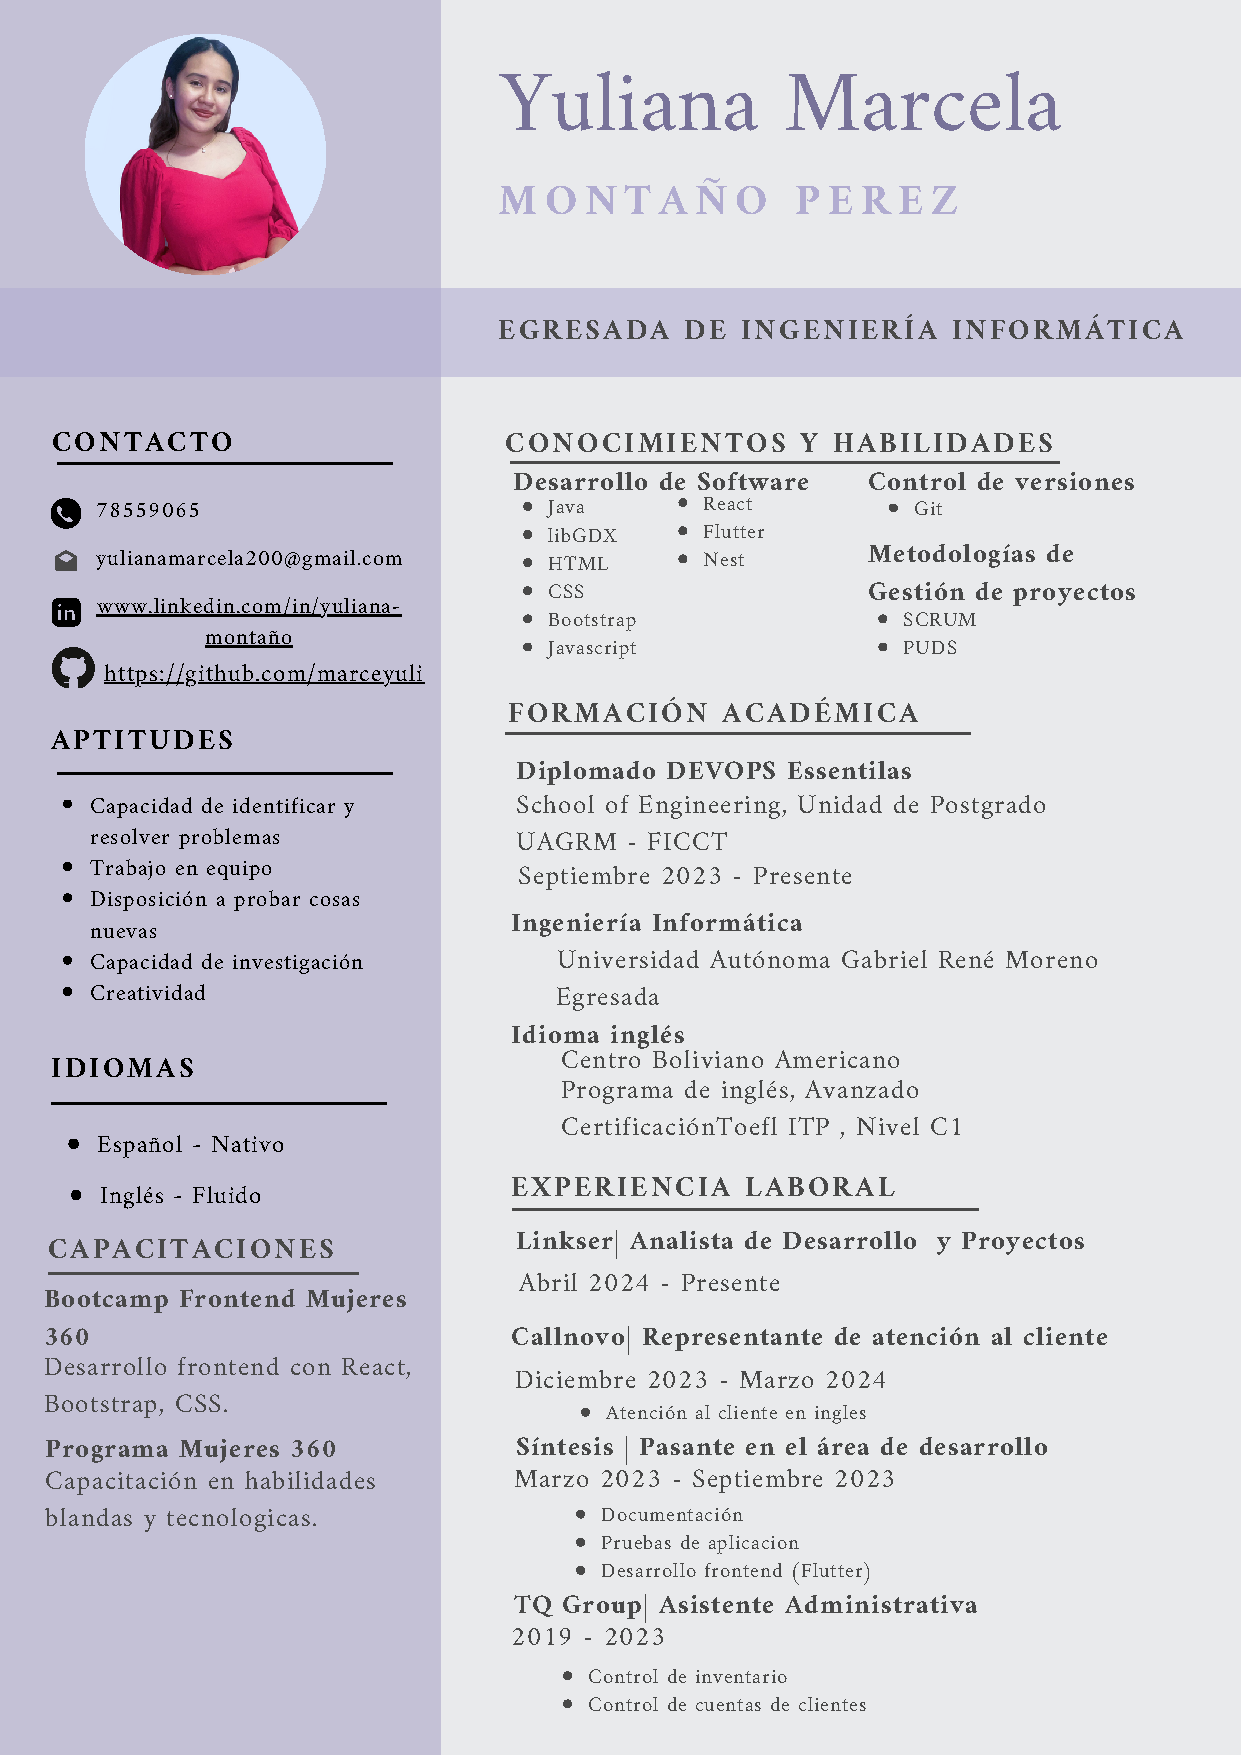
\includegraphics[width=14.5cm]{Recursos/CV.pdf}
\end{center}
\clearpage

\end{document}
